
\documentclass[runningheads]{llncs}

%\usepackage[top=1in, bottom=1in, left=1in, right=1in]{geometry}
%\usepackage{times}
\usepackage{amsmath}

%\usepackage{amsmath}
\usepackage{graphicx}
%\usepackage{setspace}
%\usepackage{subfig}
%\usepackage[hyphens]{url}
\usepackage{hyperref}
\usepackage{xspace}
\usepackage{color}
%\usepackage{flushend}
\usepackage{paralist}
\usepackage[ruled,vlined]{algorithm2e}
\usepackage{enumitem}

\usepackage{caption}
\usepackage{tabularx}
\usepackage[]{todonotes}

  
\newcommand{\sys}{Promise\xspace}
\newcommand{\discount}{\sum_{t=0}^{T} \big( \frac{\delta}{1+r} \big)^t}

\newcommand{\todoin}[1]{\todo[inline,caption={}]{#1}}
\newcommand{\toall}[1]{\todo[linecolor=orange,backgroundcolor=orange!25,bordercolor=orange,inline, caption={}]{Unassigned Todo: #1}}

\newcommand{\aza}[1]{\todo[linecolor=blue,backgroundcolor=blue!25,bordercolor=blue,inline,caption={}]{Comment by Alexei: #1}}
\newcommand{\toaza}[1]{\todo[linecolor=blue,backgroundcolor=blue!25,bordercolor=blue,inline,caption={}]{Todo for Alexei: #1}}

\newcommand{\rk}[1]{\todo[linecolor=red,backgroundcolor=red!25,bordercolor=blue,inline,caption={}]{Comment by Rami: #1}}
\newcommand{\tork}[1]{\todo[linecolor=blue,backgroundcolor=red!25,bordercolor=red,inline,caption={}]{Todo for Rami: #1}}

\newcommand{\lgu}[1]{\todo[linecolor=yellow,backgroundcolor=yellow!25,bordercolor=yellow,inline,caption={}]{Comment by Lewis: #1}}
\newcommand{\tolgu}[1]{\todo[linecolor=yellow,backgroundcolor=yellow!25,bordercolor=yellow,inline,caption={}]{Todo for Lewis: #1}}

\newcommand{\dom}[1]{\todo[linecolor=green,backgroundcolor=green!25,bordercolor=green,inline,caption={}]{Comment by Dominik: #1}}
\newcommand{\todom}[1]{\todo[linecolor=green,backgroundcolor=green!25,bordercolor=green,inline,caption={}]{Todo for Dominik: #1}}

\begin{document}

\title{
\sys: Leveraging Future Gains for Collateral Reduction
% \sys: Leveraging Future Payments for Bootstrapping Collateralized Protocols
} 
\author{
}


\date{}
\maketitle

%-------------------------------------------------
%---------------ABSTRACT------------------------
%-------------------------------------------------

\begin{abstract}
Collateral employed in cryptoeconomic protocols protects against misbehaviour of economically rational agents.
It increases the trustworthiness of a system by compensating honest users for damages using the locked capital of cheating parties.
The introduction of collateral, however, carries two disadvantages:
First, a substantial lockup requirement can act as a barrier to entry for certain protocol roles, limiting the set of candidates to wealthy agents.
Second, agents incur ongoing opportunity costs while their collateral is locked up, as it cannot be utilized elsewhere.

In this work we propose \sys, a means to decrease the initial capital requirements of a payment hub by allowing the required collateral to be constituted by future transaction fees by the user, while \emph{sustaining the overall collateral} required as a security deposit.
%We show that, using \sys, delayed payments securely held in escrow can be fairly distributed after the predefined delay.
%We further argue that \sys motivates users to lock future payments as collateral and intermediaries have higher overall collateral.
% We further show that \sys leads to a Nash equilibrium where some agent roles are motivated to lock future payments as collateral to motivate other agent roles to behave honestly without degrading the overall security provided by a system.
%\dom{Do we need that layer-two mention in there? I think Promise as a scheme is also applicable to layer 1?}
%\rk{I removed the extra layer-two word. Does interop and decentralized mining count as pure L1?}

%\dom{I was wondering about mining pools (the non-decentralized ones). But I'm not sure. I also think in Bitcoin mining you delay the payout of the reward a couple of blocks by default because of the lack of finality. What do you think?}

%\rk{It's not exactly the same, because you can initiate a transfer from the miner's wallet to a recipient immediately in the next block, right? You can play "hot potato" with the mining reward.}

Lastly, we elaborate on applying \sys to several commonly known protocols, including second-layer scaling, blockchain interoperability, and decentralized mining protocols.
\end{abstract}

%-------------------------------------------------
%---------------INTRODUCTION------------------------
%-------------------------------------------------

\section{Introduction}
\label{sec:intro}

% Alice decides between (without \sys)
% - getting p (payment)
% - getting V (payoff for cheating) - D (deposit) 
% => minimum deposit = V + p

% p > V - D

% Honest: I get p = 1 ETH => net payoff 1 ETH
% Cheating: I get V=10 ETH and I lose D=10 ETH => net payoff 0 ETH


% User: looses V but does not pay p - reimbursed D
% Op: gains V, does not get p - looses D

% Alice decides between (with \sys)
% - getting (discount_factor)^t * p
% - getting V - D
% => minimum collateral = V - (discount_factor)^t * p
% => (discount_factor)^t * p < p

% Honest: I get p = 1 discount_factor^t = 0.95 ETH
% Cheating: V=10 D=10 -> gain = 0 ETH

% D = 10 + opp.
% p = 1 - disc.

% (1*10 - disc10) - value OP gets after 10 rounds
% 10 + 10 at the start of this round available for collateral
% 10 is needed for collateral
% OP needs to lock only 1 (payoff) at round 1, V=10 (use 9 coins to get another user to pay 0.9 for round instantly)
% at round 2: 2+disc, V=10
% at round 3: 3+disc2, V=10
% at round 4: 4+disc3, V=10



% p10 = 10 - disc.*10

% opp.cost & disc. = 0.01

% Discount vs opportunity cost of locking up collateral!

% disc < opp.cost

% user pays up to (disc - opp.cost) less: f - (disc - opp.cost)

% \rk{The following sentence needs to be rephrased as to not imply that it is somehow impossible to create any protocol without an intermediary.}
When designing trustless protocols, the introduction of collateral is often necessary when an intermediary needs to be involved. %due to an impossibility of creating a protocol without an intermediary.
It allows us to create systems that are resistant against economically rational adversaries by imposing the threat of destroying their money and reinforces their honest behavior.
Collateral also provides the possibility to reimburse honest users having suffered from malicious actions of the intermediary.
Similarly, payments are a second requirement that represents a motivation for intermediaries to execute tasks requested by users in a system.
Payments and deposits are universal tools employed in protocols including cross-chain communication~\cite{Zamyatin2019XCLAIM}, scalable off-chain payments~\cite{Khalil2019NOCUST}, outsourcing of computation and verification games~\cite{teutsch2017scalable}, state channels and watchtowers~\cite{poon2016bitcoin,mccorry2018pisa}, and (decentralized) mining pools.
\dom{need citation for smartpool and p2pool}


% \subsubsection{Motivation}
% \begin{itemize}
%     \item Collateral used as universal tool to (i) incentivize correct behaviour of (trusted) intermediaries in otherwise trustless protocols and (ii) guarantee reimbursement to victim in case of failure.
%     \item Recent applications: 
%     \begin{itemize}
%         \item Cross-chain communication (XCLAIM), scalable off-chain payments (NOCUST), outsourcing of computation and verification games (TrueBit), state channels and watchtowers (Lightning Network, PISA), (decentralized) mining pools (SmartPool, P2Pool), ...
%     \end{itemize}
% \end{itemize}

\subsubsection{Challenge}
\begin{itemize}
    \item Collateral requires the intermediary to provide substantial amount of liquidity upon protocol initialization. 
    \item Initially required collateral might prove it hard for parties to participate in the protocol in the first place - especially during a bootstrapping phase of a protocol.
    \item Collateral must be at least as high as value under risk
    \item Collateral must be locked up for the duration of the protocol (can be long)
\end{itemize}

\dom{I would rather say liquidity problems and opportunity cost for locked collateral. Financial loss occurs if my collateral is lost.}
\rk{Agree with Dom}
The intermediary may hence face (i) liquidity problems and (ii) possible financial losses if funds are locked up for prolonged periods. 


\subsubsection{Intuition}
\sys helps bootstrapping cryptoeconomic protocols that require collateralized intermediaries.
Instead of requiring the intermediary to lock a high amount of collateral upfront, we require that payments made for successfully completing tasks are held in escrow for a period of time determined by a user.
Thereby, a user can start interacting with an intermediary with a small amount of value at risk and gradually increase the values by forcing the intermediary to use the ongoing payments as additional collateral.
The intermediary can withdraw surplus collateral when the sum of initially locked collateral and accrued payments is above a user defined overall collateral threshold.
That way, honest and economically rational agents have a higher net reward for behaving honest compared to locking up the collateral initially.
Also, users have the possibility to obtain a service guarantee over a defined period of time.
\dom{Let's try to find a way that compensates the intermediary for that. Maybe payment can be increased.}

Moreover, we allow users to lock future payments in escrow to reduce relative payments.
To ensure liquidity in the system, a user can lock payments, say for the expected number of tasks for a month, and in return receive a discount on the price for providing the task.
Locked future payments allow users to reduce their costs and gives intermediaries the chance to better predict demand.
In turn, locked payments motivates intermediaries to keep collateral locked in the protocol.

\subsubsection{Assumptions}
In \sys, a user Bob engages an intermediary Alice to fulfill a task on his behalf.
Alice provides a deposit to prevent her from behaving malicious and receives a payment for successfully completing the task.
We assume that Alice is an economically rational agent.
Also, we assume that the protocol utilising \sys implements payments and deposits through a distributed ledger that provides the functionalities as describes in, e.g.~\cite{Badertscher2018Genesis}.
The payment and the deposit are held in custody by a smart contract implemented within the decentralized ledger.
Further, there is a one to one mapping between the collateral and a user, i.e.\ the collateral of an intermediary is not split between multiple users.
Last, agents in the system can be identified with their public/private key pair.

\subsubsection{Structure}
We introduce the general model in Section~\ref{sec:model} followed by describing the \sys protocol in Section~\ref{sec:promise}.
Next, we discuss the security of \sys in Section~\ref{sec:security} and present how to apply the protocol to existing systems in Section~\ref{sec:application}.
Related work is introduced in Section~\ref{sec:related}.
We conclude in Section~\ref{sec:conclusion}.


%-------------------------------------------------
%---------------MODEL------------------------
%-------------------------------------------------


\section{Model}
\label{sec:model}

\rk{Would it make sense to rename $D_{min}$ to $D_{base}$? Minimum sort of implies that it's already minimized while base can refer to a base value Promise optimizes.}

Assume that we have two agents: Alice, an intermediary, and Bob, a user.
For a generic service, Alice and Bob agree on a contract that details which task Alice has to provide in a specification $\phi$.
Bob will pay Alice $p$ each period $t$ for fulling the task.
The generic service typically implies a requirement that the value of the task is ``insured'' via a deposit $D$.
For instance, Bob may enlist Alice to perform an atomic swap for funds of total value $V$, offering a payment $p$ for this service, where $p<V$.
\rk{"such that $D_{min} \geq V$". Not a general statement for all protocols we consider though.}
In this case, Alice usually has to provide a minimum amount of collateral $D_{min}$ upfront, such that $D_{min} \geq V$.
Further, Bob provides exactly the next payment $p_i$ into an escrow.
Upon successful completion and verification of the task, Alice can withdraw the payment and the deposit.

\subsection{\sys}
In \sys, we propose two changes to this procedure.

\begin{enumerate}
    \item Alice is able to reduce the initially provided collateral from $D_{min}$ to $D_I$ such that $D_I < D_{min}$. Over time, Alice is able to to accumulate an amount of collateral $D \geq D_{min}$ by keeping her payments $p_i$ in escrow. Alice can withdraw surplus collateral if (i) the payments or initial collateral have been in escrow for more than a period $t \geq \tau$, and (ii) her current collateral is higher than the minimum requirement $D_{min}$. This eases the upfront collateral burden on Alice.
    \item Bob is able to lock multiple future payments $\{p_1, ..., p_n\}$ in escrow. This allows Bob to reduce transaction costs and effectively have a subscription option on the provided service.
\end{enumerate}

\subsection{Roles}

Promise adopts the BAR model of rational agents~\cite{aiyer2005bar} with the extensions proposed in Balance that include private preferences of agents~\cite{Harz2019Balance}.
Given this model, we define the following roles in \sys.

\begin{itemize}
    \item \textbf{Alice}, the Intermediary: Alice is an economically rational agent that is entrusted with executing a task in a protocol. She provides a deposit $D$ into the escrow before executing the task and receives a payment $p$ when successfully completing a task.
    \item \textbf{Bob}, the User: Bob represents the user requesting execution of a task by Alice as defined in the specification $\phi$. A user provides payments $\{p_1, ..., p_n\}$ into the escrow. Bob can provide multiple future payments into the escrow.
    \item \textbf{Escrow}: The escrow is a smart contract responsible for holding deposits by Alice and payments by Bob. Further, Bob's future payments are also stored in the escrow.
    \item \textbf{Verifier}: The verifier checks the behavior of Alice as defined in the specification. In practice, this can be a smart contract, a dedicated third party, or the user.
\end{itemize}


\dom{Do we need to define blockchain model with finality assumptions, parameter $k$ etc.?}
% \subsection{Utilities}

% Parameters
% \begin{itemize}
%     \item $A$: Intermediary Alice
%     \item $B$: User Bob
%     \item $u$: utility
%     \item $p$: payments
%     \item $p_{lock}$: locked payments
%     \item $p_{future}$: future payments provided in advance
%     \item $\tau$: payment lock-up period
%     \item $D$: total deposit ($D_I + D_P$)
%     \item $D_I$: initial deposit
%     \item $D_P$: accumulated deposit $\sum_i^{P} p_{lock}$
%     \item $c$: cost
%     \item $v$: private valuation (preference)
%     \item $\mathrm{E}[r]$: expected rate of return (expressing opportunity cost)
%     \item $t$: time step
%     \item $T$: period length
%     \item $\delta$: discount factor
% \end{itemize}


\subsection{Bob's payments}






% \dom{Need this for the security analysis}

% Alice utility
% \begin{equation}
%     u_A(\sigma_A) =
%     \begin{cases}
%         p-c_A- \discount \mathrm{E}[rD_A], & \text{if } \phi(\sigma_A) = 1 \\
%         v_A - D_A - c_A - \discount \mathrm{E}[rD_A], & \text{if } \phi(\sigma_A) = 0 \\
%     \end{cases}
% \end{equation}

% Bob utility:
% \begin{equation}
% \label{eq:receiverutil}
% u_B(\sigma_A) =
%     \begin{cases}
%         v_B-p-c_B - \discount \mathrm{E}[rp], & \text{if } \phi(\sigma_A) = 1 \\
%         D_A-v_B-c_B - \discount \mathrm{E}[rp], & \text{if } \phi(\sigma_A) = 0 \\
%     \end{cases}
% \end{equation}

% The specification is verified by the verifier, represented either by a smart contract or a third party.
% \dom{Add examples here}.



% ``Active'' and ``passive'' collateral.

%-------------------------------------------------
%---------------PROTOCOL------------------------
%-------------------------------------------------


\section{Promise}
\label{sec:promise}

\begin{figure}
    \centering
    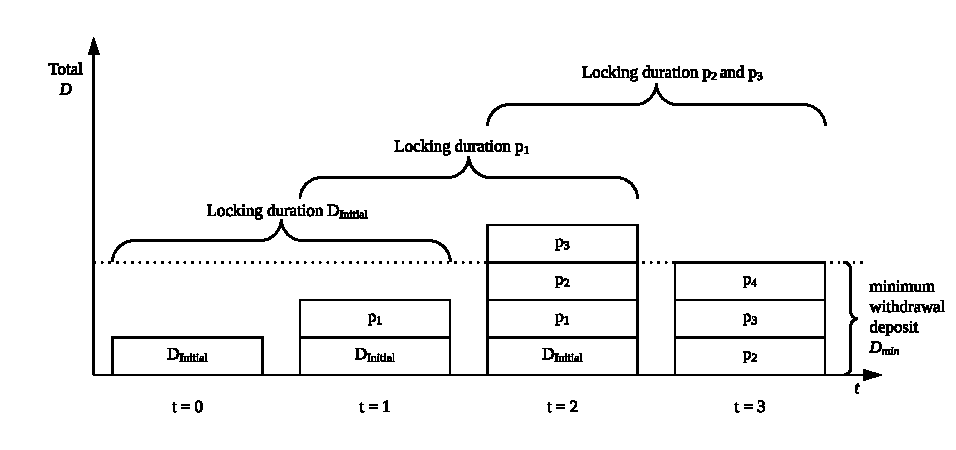
\includegraphics[width=\textwidth]{promise/figures/Promise.pdf}
    \caption{\sys allows intermediaries to lock-up less initial deposit $D_I$ and use payments $p_i$ as additional deposit. The initial deposit and payments are locked for a period of time $\tau$. If the time period has passed and the agent has more collateral than the minimum requirement $D_{min}$, the agent can withdraw surplus collateral. In this example, at $t=0$ the intermediary Alice provided $D_I$ as the initial deposit, which is locked for two time steps (i.e.\ becomes free at $t=3$). At $t=1$, Bob pays Alice for executing a task with $p_1$ which is stored as additional collateral. At $t=2$, Alice receives two more payments from Bob, $p_2$ and $p_3$ which bring her total collateral above the minimum requirement $D_{min}$. At $t=4$ Alice is allowed to withdraw an amount equal to $D_I + p_1$ as both the locking period of these have passed and with $p_4$ Alice's overall collateral is at least equal to the minimum collateral requirement.}
    \label{fig:promise}
\end{figure}


\begin{enumerate}
    \item Abstract protocol definition
    \begin{itemize}
        \item Use rewards that are guaranteed to be received in the future (i.e., already earned) to reduce the amount of active collateral locked in the smart contract.
    \item Requirement: identities of participants. But, this also contributes participants not Sybil-attacking the system.
    \end{itemize}
    \item Distinction between the two instances (user vs operator must lock up collateral)
    \begin{itemize}
        \item Prevention of user misbehavior: users join the system and lock up collateral, participate in the protocol correctly and earn future rewards. The longer they behave correctly, the more passive collateral they accumulate - and the less active collateral they need to keep locked in the system. This goes up to some bound. This is used in PPLNS mining pools.
        \item Prevention of operator misbehavior: operator charges users fees but keeps this money in the contract as passive collateral. If he behaves correctly, he will receive these funds after some delay. Users pre-pay the operator for a period $t$ and the operator then uses these funds to reduce the active collateral has to provide for the protocol.
        An option here is for users also to build up the fees gradually (just like in the PPLNS case) - the more the users use the system, the more fees are locked, and the less active collateral the operator must allocate for that user.
    \end{itemize}
\end{enumerate}

\section{Model as of 18 September}

\subsection{The setup}

Consider the following setup.

\begin{itemize}
    \item an operator, Alice, who can offer a collateralized service for off-chain payments. This service can offer a varying degree of instant finality. 
    \item $n$ users, including Bob, who wish to make and receive payments. 
    \item each user pays a fee $p$ per inbound transaction (assumed to be the same size each period for simplicity.
\end{itemize}

Alice has a choice between two actions: acting honestly, or cheating. 
With \sys, the payoffs to Alice of each of these actions are as follows.
Assume that any cheating happens at period $t=T$.

\dom{Why is the deposit added to the payoff when being honest? Before the protocol started, the deposit was already in the account of the operator. So his net profit is only the payment.}
\begin{equation}
\label{eq:promise_honest}
\Pi_H = D(\frac{\delta}{1+r})^T+p\sum^{T}_{t=0}(\frac{\delta}{1+r})^t
\end{equation}

\dom{Why do you subtract the payment from the payoff for cheating? Before the protocol started, the operator did not have the payment in his account. He will not receive the payment, but that does not mean that he has to pay an amount equal to the payment into the system.}

\begin{equation}
\label{eq:promise_cheat}
\Pi_C = V-D(\frac{\delta}{1+r})^T-p\sum^{T}_{t=0}(\frac{\delta}{1+r})^t
\end{equation}


\dom{
Let's take an example where Alice (operator) starts with a balance of 10 ETH and Bob starts with a balance of 10 ETH and has multiple goods with value 15 ETH each. 
For simplicity, I will not consider any discount factors or opportunity costs.
Bob is willing to pay Alice 1 ETH per transaction, i.e. one transfer of the good.
In the first of those transaction Alice posts 10 ETH as collateral, she now has a balance of 0 ETH (-D).
Bob then pre-pays 10 ETH to pay for the transactions. Bob has a balance of 0 ETH (-q).
The escrow contract has 20 ETH now.
Alice has two choices.
\begin{itemize}
    \item Honest: Alice is honest and the good is transferred successfully. Alice and Bob still have 0 ETH in their accounts. If we would finish the transactions at this point, Alice would get her deposit back and the payment for one transaction (even after some time) and Bob would get the remainder from his pre-payment out. Alice would have 11 ETH and Bob 9 ETH. \textbf{Alice went from 10 ETH to 11 ETH. The equation for honest behaviour is therefore $u = p$ (or $\Pi_H=p$ in the notation above).}. Again without considering the discount factor. Alice does not get any surplus deposit.
    \item Cheating: Alice decides to steal the good from Bob. Alice and Bob still have 0 ETH in their accounts. Let's say Alice is able to sell the good directly at the market price of 15 ETH. In that case Alice has 15 ETH in her account. Bob get's the transaction refunded from the contract and his payments back. Bob get's the 10 ETH deposit from Alice and the 10 ETH he put in as payment. \textbf{Alice has made a plus of 5 ETH (-10 ETH deposit + 15 ETH of $V$, resulting in the equation $u = V - D$ (or $\Pi_C=\Gamma - D$ in the notation above). Alice never had the payment and it is not her loss to not receive it. She decides on purpose against receiving a payment because the net payoff of cheating (+5 ETH) is higher than being honest (+1 ETH).}
\end{itemize}
}
\dom{I think at this point our assumptions might diverge. In my opinion Alice could now go ahead and create a Sybil identity and try to cheat on Bob again and steal the good. I'm proposing a new model below that I think works, but might be different from what you have in mind.}

%-------------------------------------------------
%---------------Security------------------------
%-------------------------------------------------

\section{New model proposal}
\subsection{Variables}
\begin{itemize}
    \item $A$: Intermediary Alice
    \item $B$: User Bob
    \item $\gamma$: Bob's exit probability. If Bob is cheated on there is a probability that Bob will not use the system any longer.
    \item $u$: utility
    \item $p$: payment
    \item $m$: multiplier for future payments, for example $mp$ means $m$ times $p$ payments provided in advance
    \item $\tau$: payment lock-up period
    \item $D$: total deposit ($D_I + D_P$)
    \item $D_I$: initial deposit
    \item $D_P$: accumulated deposit $\sum_i^{P} p_{lock}$
    \item $c$: cost
    \item $V$: private valuation (preference) of an outcome. Bob can use this to value the transfer. Most importantly, it is the value that Alice sets for being a cheater.
    \item $\mathrm{E}[r]$: expected rate of return (expressing opportunity cost)
    \item $t$: time step
    \item $\delta$: discount factor
    \item $r$: rate of return
\end{itemize}

\subsection{Basic case}
Alice is the intermediary.
Bob uses the service provided by Alice.
Alice has a known incentive to cheat in the protocol $V$.
$V$ presents her monetary payoff for cheating and is known in advance.
In a typical protocol the deposit $D$ needs to be set equal to $V$ to prevent Alice from cheating.

In \sys, Alice stakes some amount of deposit $D_I$ where $D_I < V + p$.
Bob has a probability $\gamma$ that he will leave the protocol for good if he is cheated on.
The more often he is cheated on the higher the probability that he will leave the protocol.

Bob is going to pre-pay for the service by a factor $m$, such that $mp$ coins are hold in the escrow.
Bob is able to receive $m$ times the service from Alice.
Alice is either paid all $mp$ coins or none, if Alice cheats at any point in the protocol.
Further, Alice's payment is delayed by a factor $\tau \geq m$, i.e.\ Alice is earliest paid when the whole contract is finished.

For simplicity of argument, $p$ remains constant over time.
Also, for simplicity we will not include discount factors on future payments and opportunity costs for now.

Assume that Alice has provided her deposit $D_I$ and Bob has made the prepayment $mp$.
At $t=0$, Alice is confronted with two choices.
\begin{itemize}
    \item Honest: If Alice makes the honest choice for this round, she might receive a payoff of $u=mp$ after a time $m+\tau$ has passed (would need to be discounted).
    \item Cheating: If Alice cheats, she looses the deposit but gains her incentive to cheat such that $u=V-D$.
\end{itemize}

Since we require a all or nothing strategy from Alice and Bob, we increase the incentive to be honest from $p$ to $mp$.

\subsection{Sybil identities}
However, Alice could still gain from this.
If we assume that in every round, Alice is able to make a higher profit from cheating, i.e.\ $p < V -D$ holds, Alice would just cheat Bob every round.
In this case, Alice does not care that Bob introduced the $m$ factor to the payment, because Bob just comes back as a naive customer to be cheated again.
However, we assume that Bob is a bit smarter than that.
Bob only comes back with a probability $0 < \gamma < 1$.
Alice needs to consider that even with a Sybil identity, there will at some point be no users left to cheat since no-one is using the system any longer.

Adding the probability parameter leaves Alice with the choice between:
\dom{This is not correct yet. Need to think how to in-cooperate that. As long as Alice can be reasonable sure that she can cheat once on Bob, Alice can cheat in the first round and then in the second serve Bob as a regular operator without cheating on him.}
\begin{align}
    u_H &= \frac{1}{\gamma} p \\
    u_C &= \gamma (V - D)
\end{align}


\section{Security Analysis}
\label{sec:security}

We argue about the security of adding \sys to an existing protocol.
\sys aims to fulfil the following security properties:

\begin{enumerate}
    \item \textbf{Payment and deposit safety}: Payments $p$ (future and current) provided by a user as well as deposits $D$ by intermediaries cannot be stolen.
    \item \textbf{}
\end{enumerate}

\subsection{Incentive arguments}
\dom{Personal playground for now ;)}


Say preference for intermediary to cheat is $v$.
Provided deposit is $D_I < D_{min}$.
Without \sys, provided deposit is $D_{min}$.
Let's say $v = D_{min}$, i.e.\ 100\% collateralization ratio.

\subsubsection{Single-round game}
Assuming a protocol without \sys.
If Alice cheats, she gets $u = v - D_{min} = 0$.
If Alice is honest, she gets $u = p$.
Without \sys, Alice should not cheat in a single round game.

Assuming a protocol with \sys:
If Alice cheats, she gets $u = v - D_I > 0$
If Alice is honest, she gets $u = (\frac{\delta}{1+r})^{\tau} p$
For Alice not to cheat in a system with \sys in a single-round setting, we require:

\begin{equation}
    \big( \frac{\delta}{1+r} \big)^{\tau} p > v - D_I
\end{equation}

Consequences:
\begin{itemize}
    \item Safely reducing the initial collateral from $D_{min}$ to $D_I$ is bound to $D_I = D_{min} - (\frac{\delta}{1+r})^{\tau} p$.
    \item Assuming $\delta < 1$ and $r \geq 1$, the larger $\tau$, the less initial reduction is possible.
    \item The lower $\delta$ the less reduction.
    \item The higher $r$, the less reduction.
\end{itemize}

\subsubsection{Sequential game}
Assuming a protocol without \sys.
If Alice cheats, she gets $u = \sum_{t=0}^{\infty} \big( \frac{\delta}{1+r} \big)^{t} (v - D_{min}) = 0$.
If Alice is honest, she gets $u = \sum_{t=0}^{\infty} \big( \frac{\delta}{1+r} \big)^{t} p > 0$.
Without \sys, Alice should not cheat in a sequential game.

Assuming a protocol with \sys:
If Alice cheats, she gets $u = \sum_{t=0}^{\infty} \big( \frac{\delta}{1+r} \big)^{t} (v - D_{I}) > 0$
If Alice is honest, she gets $u = \sum_{t=0}^{\infty} \big( \frac{\delta}{1+r} \big)^{t} (\frac{\delta}{1+r})^{\tau} p$
For Alice not to cheat in a system with \sys in a single-round setting, we require:



\subsection{User protocol part}
Basic argument:
if user pays every round $t$ then his net utility per round is $u = v - p - c$ where $v$ is his private value for getting the service, $p$ the payment he makes and $c$ the cost for doing the payment.
Locking multiple payments incurs opportunity cost $\big( \frac{\delta}{1+r} \big)^t \mathrm{E}[rp]$ at every time step $t$.
The user should lock future payments such that his utility is increased.
If we make a sequential game of this, the utility is defined by the number of rounds $m$ the user wishes to participate (no pre-payment):

\begin{align}
\label{eq:utility-user-no-prepay}
    u &= \sum_{t=0}^{m} \big( \frac{\delta}{1+r} \big)^t (v - p - c)
\end{align}

With pre-payment, we have:

\begin{align}
\label{eq:utility-user-prepay}
    u &= v - p - c + \sum_{t=1}^{m} \big( \frac{\delta}{1+r} \big)^t (v - p - \mathrm{E}[rmp])
\end{align}

If the overall utility to pre-pay is higher, then a user should do so, even if the user does not expect to transfer higher values $v$ in subsequent transactions.
Hence, we equate Eq. (\ref{eq:utility-user-no-prepay}) and (\ref{eq:utility-user-prepay}) to determine the decision bound.

\begin{align}
    c = \mathrm{E}[rmp]
\end{align}

Realistically, $r$ is in between $0$ and $0.05$ reflecting a maximum of a 5\% return in another protocol.
Plugging in the maximum value for $r$ gives us the following plot.




\subsection{Notes}
Define 3 security properties here and argue that they hold. 


\begin{itemize}
    \item Passive collateral cannot not be stolen
    \item Promise is incentive compatible
    \begin{itemize}
        \item Increase the amount of locked-up capital by the intermediary to prevent cheating
        \item Reduce the opportunity cost for the intermediary
        \item End users should not suffer additional opportunity cost from this
    \end{itemize}
\end{itemize}

Mapping of collateral to multiple users is Sybil attack-able. Intermediary can create identities that will receive part of the collateral if he is slashed.

%-------------------------------------------------
%---------------APPLICATION------------------------
%-------------------------------------------------


\section{Applications}
\label{sec:application}

High level desc. of applications + how \sys can be applied.
Suggestions:
\begin{itemize}
    \item NOCUST
    \item XCLAIM
    \item SmartPool
    \item What else? PISA, MakerDAO, Stablecoins, ...
\end{itemize}

%-------------------------------------------------
%---------------RELATED WORK------------------------
%-------------------------------------------------


\section{Related Work}
\label{sec:related}

Relate to finance.

\tolgu{Add related work from finance. The principle of pre-payment is not new, but only with smart contracts we can actually provide some guarantees that the funds will be returned to the users in if there is no misbehavior, i.e. cannot be stolen.}


Other related work?
\todom{Can you cover this? Does not have to be much, we have limited space.}
\begin{itemize}
    \item Balance
    \item New paper by Teutsch
    \item Payment streaming \url{https://github.com/ethereum/EIPs/issues/1620}
\end{itemize}

%-------------------------------------------------
%---------------CONCLUSION------------------------
%-------------------------------------------------

\section{Conclusion}
\label{sec:conclusion}


\bibliographystyle{splncs04}
\bibliography{bib/blockchain,bib/references}

\end{document}
